\documentclass[tikz]{standalone}
\usetikzlibrary{positioning, arrows.meta}
\begin{document}
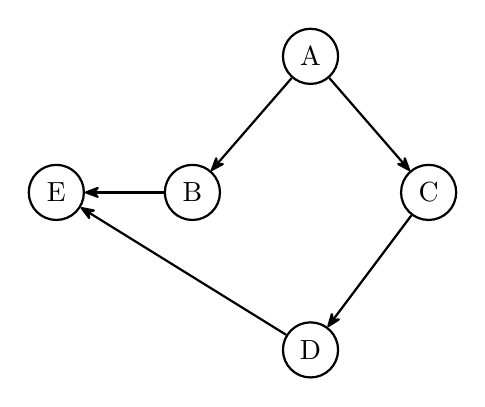
\begin{tikzpicture}[ roundnode/.style={circle,draw=black, thick, minimum size=7mm}]
\node[roundnode]        (uppercircle)        {A};
\node[roundnode]        (lowercircle)       [below=of uppercircle, xshift=-15mm] {B};
\node[roundnode]        (leftcircle)        [below=of uppercircle, xshift=+15mm]{C}; 
\node[roundnode]        (effect)            [left=of lowercircle]{E};
\node[roundnode]        (some)              [below=of uppercircle, yshift=-20mm] {D};
\draw[->, >={Stealth[round]}, thick] (uppercircle) to (lowercircle);
\draw[->, >={Stealth[round]}, thick] (uppercircle) to (leftcircle);
\draw[->, >={Stealth[round]}, thick] (lowercircle) to (effect);
\draw[->, >={Stealth[round]}, thick] (leftcircle) to (some);
\draw[->, >={Stealth[round]}, thick] (some) to (effect);
\end{tikzpicture}
\end{document}
